\title{Midterm Study Guide - INTD290}
\author{Dr. Jordan Hanson - Whittier College Dept. of Physics and Astronomy}
\date{\today}
\documentclass[10pt]{article}
\usepackage[a4paper, total={18cm, 27cm}]{geometry}
\usepackage{outlines}
\usepackage{hyperref}
\usepackage{graphicx,subfigure}
\begin{document}
\maketitle

\section{How to Use this Study Guide}

\begin{enumerate}
\item Material not on this study guide is usually not covered on the midterm.
\item The midterm will typically be more detailed, but this study guide shows you the areas you should know.
\item The midterm will have the same \textit{style} and \textit{structure} of this study guide.
\end{enumerate}

\section{Maps of The New World}

\begin{figure}[ht]
\centering
	\subfigure[Virreinato 1]{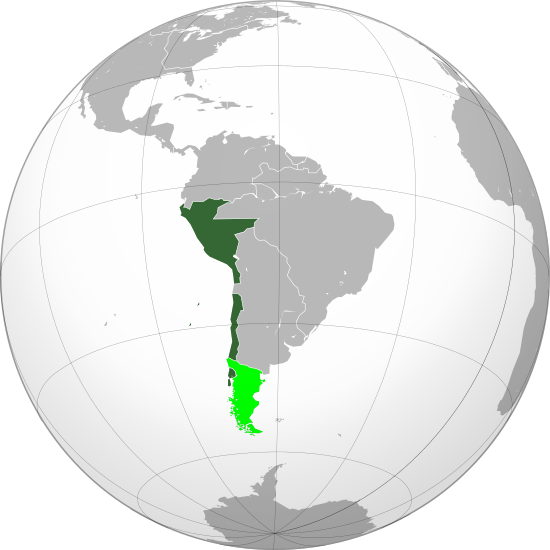
\includegraphics[width=0.2\textwidth]{figures/vice_peru.png}}
	\subfigure[Virreinato 2]{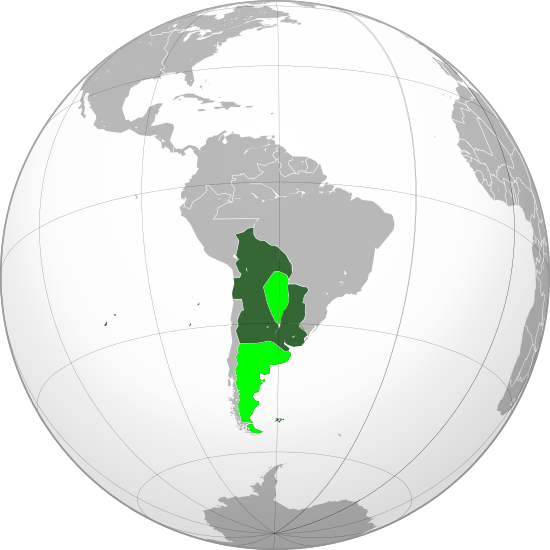
\includegraphics[width=0.2\textwidth]{figures/vice_riodelaplata.png}}
	\subfigure[Virreinato 3]{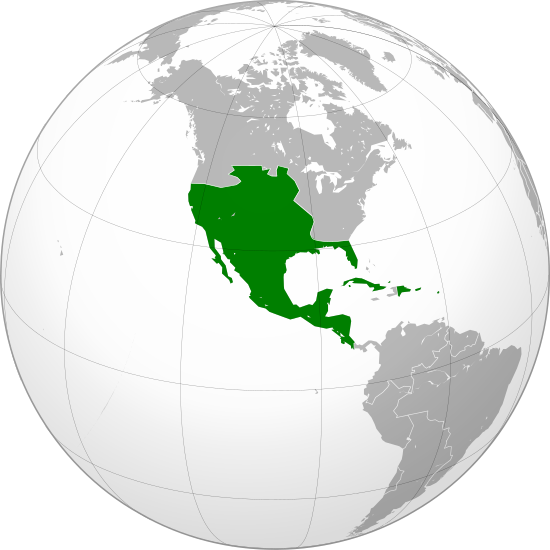
\includegraphics[width=0.2\textwidth]{figures/vice_nuevaespana.png}}
	\subfigure[Virreinato 4]{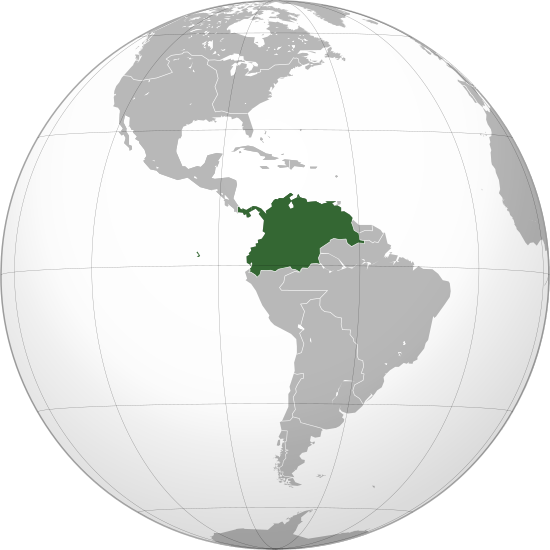
\includegraphics[width=0.2\textwidth]{figures/vice_nuevagranada.png}}
\caption{\label{fig:map1} There were up to four \textit{virreinatos} during the Spanish colonial period of Latin American history.}
\end{figure}

\begin{enumerate}
\item In which of the four \textit{virreinatos} of the Spanish colonial empire (shown in Fig. \ref{fig:map1}) was the language \textit{Nahuatl} spoken?
\item In which of the four \textit{virreinatos} had the city of Lima as its capital?
\item Which two of the four \textit{virreinatos} were at one point one kingdom?
\item In which of the four \textit{virreinatos} was crucial data on the transit of Venus in 1789 collected?
\item Recall the story of the famous silver mines of \textit{Potos\'{i}}.  In which \textit{virreinato} is the \textit{cerro rico} located?
\item There is a city within one of the four \textit{virreinatos} that had the following four colleges/univerisities \textit{circa 1774}: \textit{Universidad de Santo Tom\'{a}s}, \textit{Colegio Mayor del Rosario}, \textit{Colegio Mayor del Bartolom\'{e}}, and \textit{Universidad de San Nicol\'{a}s de Bari}.  The University of Saint Thomas (\textit{San Tom\'{a}s}) was at various times controlled by the Dominican order (Saint Thomas Aquinas was a Dominican).  What is the city and in which \textit{virreinato} is it?
\item Which \textit{virreinato} had Buenos Aires as its capital?  What are some reasons it would have been convenient to have a capital city located there, geographically speaking? \\
\end{enumerate}

\clearpage

\section{Asynchronous Activity Review I}

\begin{figure}
\centering
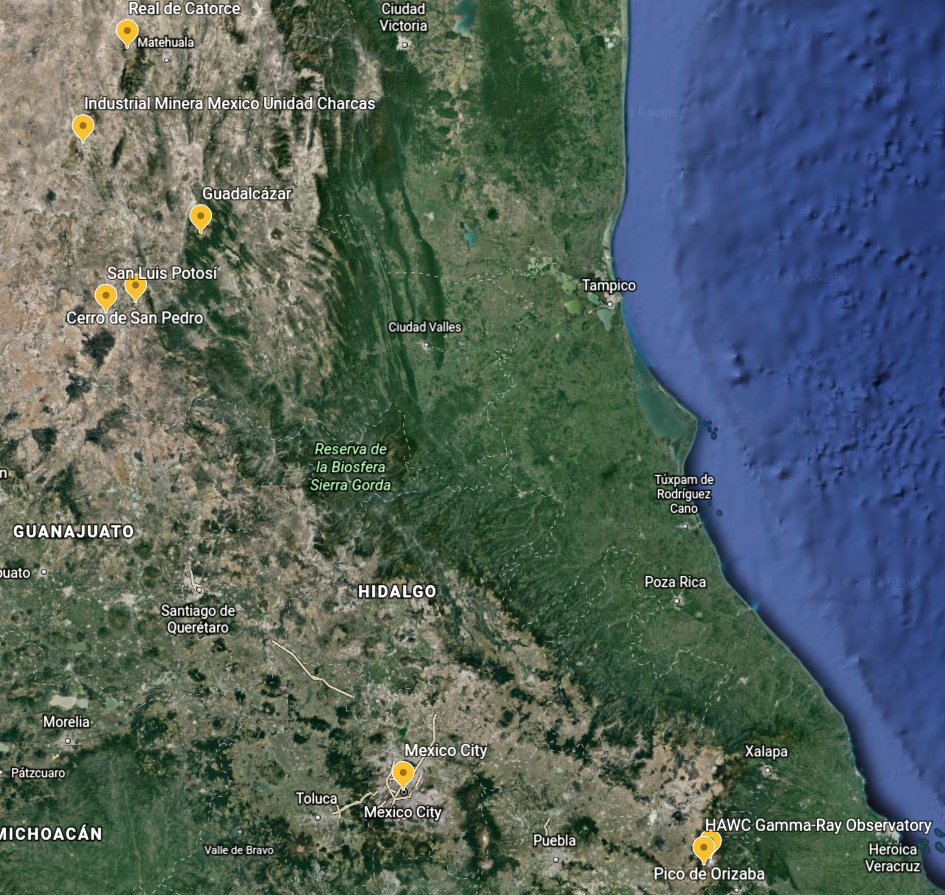
\includegraphics[width=0.6\textwidth]{figures/mines.png}
\caption{\label{fig:mines} A section of the map of modern day Mexico.}
\end{figure}

\begin{enumerate}
\item What is the historical signficance of the five locations to the Northwest in Fig. \ref{fig:mines}, in terms of the formation of colleges and universities in colonial Mexico? \\ \vspace{2cm}
\item Approximately when were these places founded as towns and cities?  What was the principle economic sector at the time? \\ \vspace{2cm}
\item \textbf{Connection to modern science:} In the Southeast side of Fig. \ref{fig:mines}, there is a physics detector located near Pico de Orizaba.  What does it detect, and how does it work? Can you draw a diagram showing how one of the components functions? \\ \vspace{2cm}
\end{enumerate}

\clearpage

\section{Asynchronous Activity Review II}

\begin{figure}[hb]
\centering
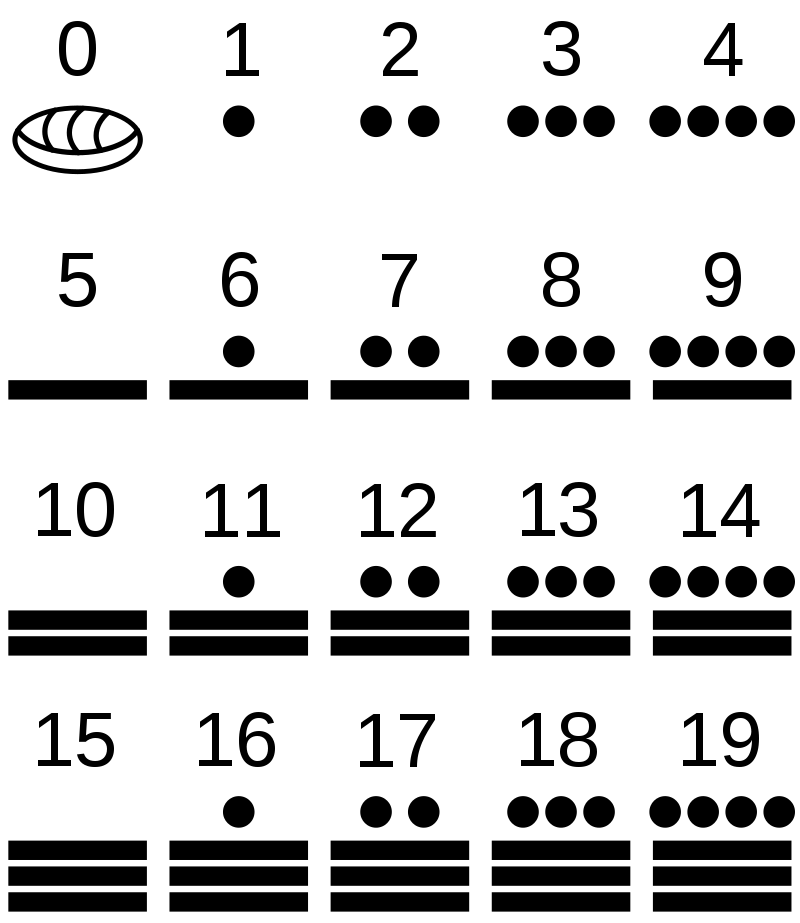
\includegraphics[width=0.2\textwidth]{figures/maya_digits.png}
\caption{\label{fig:digits} A list of the numerical digits used by the Maya.}
\end{figure}
\begin{enumerate}
\item Work out the following addition problems \textit{using the Mayan system.}
\begin{enumerate}
\item $21 + 21 = $ \vspace{2cm}
\item $425 + 425 = $ \vspace{2cm}
\item $4096 + 2048 = $ \vspace{2cm}
\end{enumerate}
\item Work out the following subtraction problems \textit{using the Mayan system.}
\begin{enumerate}
\item $4096 - 2048 = $ \vspace{2cm}
\item $56 - 47 = $ \vspace{2cm}
\end{enumerate}
\item Work out the following addition problems \textit{using the Incan quipu:}
\begin{enumerate}
\item $42 + 42 = $ \vspace{2cm}
\item $256 + 128 = $ \vspace{2cm}
\end{enumerate}
\item Work out the following subtraction problems \textit{using the Incan quipu:}
\begin{enumerate}
\item $42 - 21 = $ \vspace{2cm}
\item $256 - 128 = $ \vspace{2cm}
\end{enumerate}
\item Suppose you have three terrace plots in the Andean mountains to use to survive.  You and your cohort of fellow Incans decide to grow potatoes and lima beans\footnote{Pinto beans, for example, take too long to grow at these altitudes, and boiling them is difficult at high altitude because water boils at lower temperatures.}. Suppose a potato plant requires a 0.25 meter by 0.25 meter patch of land, and a lima bean plant requires a 0.1 meter by 0.1 meter patch.  If you decide to use one terrace for potatoes, and two for lima beans, and each terrace is 20 meters by 10 meters, how many potato plants and how many lima bean plants can you plant? Show the work in Incan Quipu style.  \\ \vspace{4cm}
\end{enumerate}

\section{Connection to Physics}

\begin{figure}
\centering
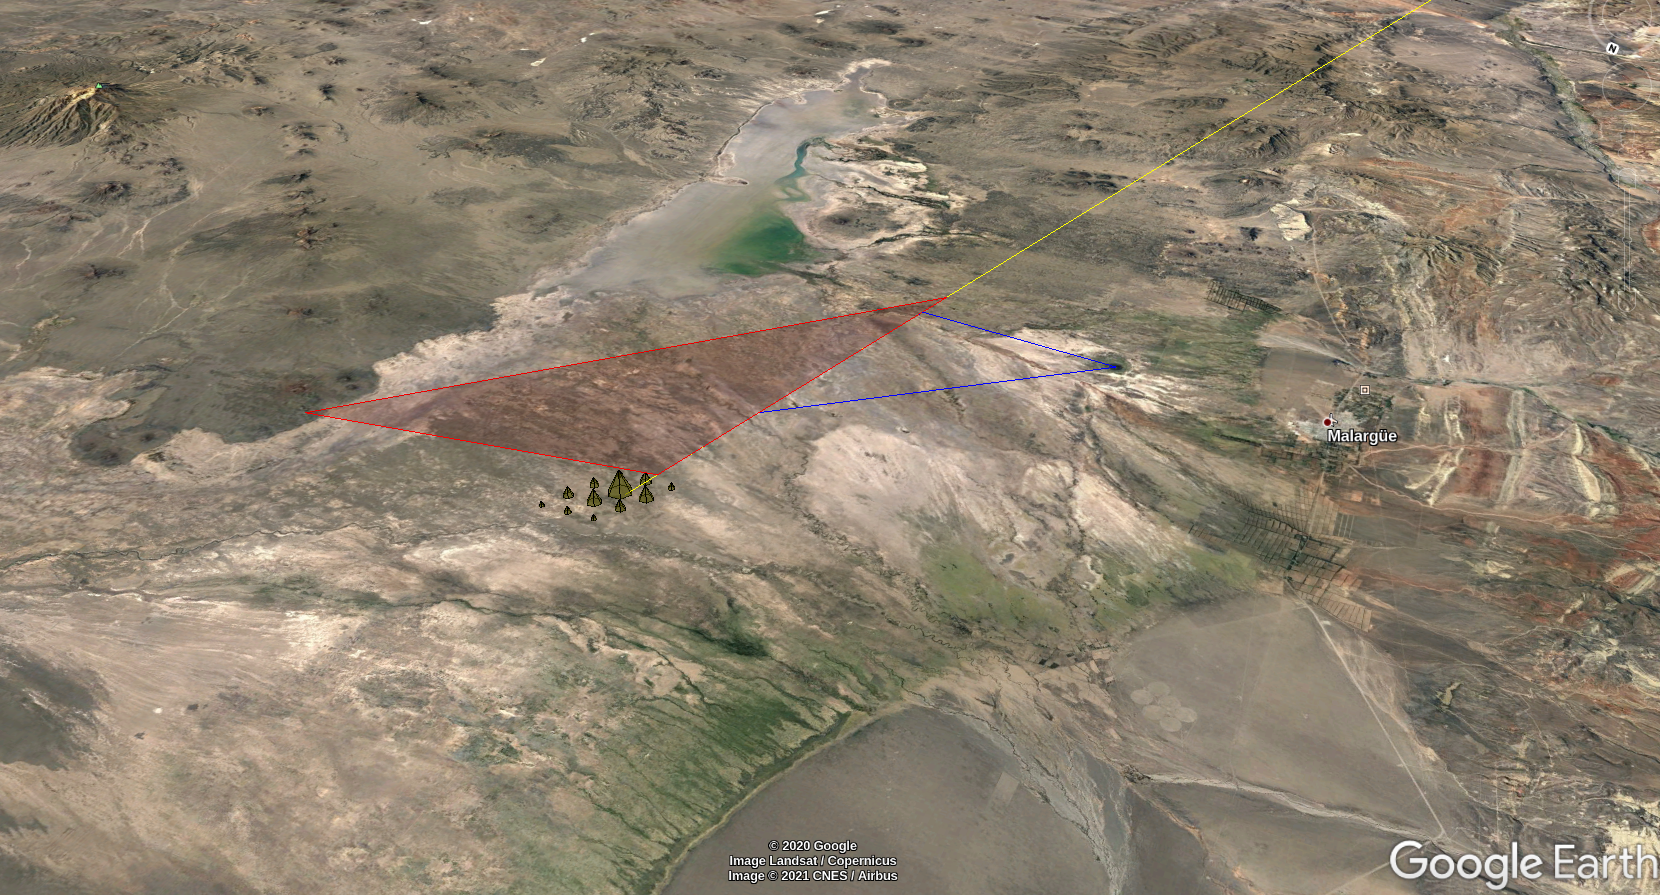
\includegraphics[width=0.7\textwidth]{figures/auger.png}
\caption{\label{fig:auger} A map of a \textit{cosmic ray} event hitting the Pierre Auger Observatory, near Malarg\"{u}e}
\end{figure}

\begin{enumerate}
\item In Fig. \ref{fig:auger}, a \textit{cosmic ray} is shown hitting detectors in the Pierre Auger Observatory (PAO).  In what country is the PAO?
\begin{itemize}
\item A: Chile
\item B: Mexico
\item C: Argentina
\item D: Bolivia
\end{itemize}
\clearpage
\item What is a cosmic ray?
\begin{itemize}
\item A: A photon of light
\item B: A proton or nucleus from deep space
\item C: A portion of the aurora borealis
\item D: An ion floating in the atmosphere
\end{itemize}
\item To what does the yellow line in the sky correspond?
\begin{itemize}
\item A: The direction of the cosmic ray
\item B: The energy of the cosmic ray
\item C: The charge of the cosmic ray
\item D: The speed of the cosmic ray
\end{itemize}
\item Cosmic rays make a shower of other radioactive particles when they smash into the atmosphere.  To what do the brown pyramids on the ground correspond?
\begin{itemize}
\item A: Where the cosmic ray shower hits the Earth
\item B: The energy or number of particles in the shower
\item C: The speed of the shower particles
\item D: A and B
\end{itemize}
\end{enumerate}

\section{Vocabulary}

\begin{enumerate}
\item What is the meaning of the term \textit{empiricism?}
\begin{itemize}
\item A: Relying on pure reason to gain knowledge
\item B: Encapsulating the idea of \textit{I think, therefore I am.}
\item C: Using scientific instruments
\item D: Relying on measurements and sensory experience to discover the truth
\end{itemize}
\item What is the meaning of the term \textit{Cartesian coordinates?}
\begin{itemize}
\item A: The connection between geometry and algebra
\item B: Measuring locations and distances with numbers in directions perpendicular to each other
\item C: Equivalent to the Pythagorean theorem
\item D: A and B
\end{itemize}
\item What is the meaning of the \textit{Nahuatl} term \textit{altepetl?}
\begin{itemize}
\item A: A man
\item B: A family
\item C: A town
\item D: A nation
\end{itemize}
\item What is the meaning of the \textit{Nahuatl} term \textit{chilpoctli?}
\begin{itemize}
\item A: Smoked fish
\item B: Smoked chili
\item C: An herb to help digestion
\item D: A mountain
\end{itemize}
\item What is the meaning of the \textit{Nahuatl} term \textit{chilpoctli?}
\begin{itemize}
\item A: Smoked fish
\item B: Smoked chili
\item C: An herb to help digestion
\item D: A mountain
\end{itemize}
\item What is the meaning of the \textit{Nahuatl} term \textit{huitzilin?}
\begin{itemize}
\item A: An otter
\item B: A falcon
\item C: A condor
\item D: A hummingbird
\end{itemize}
\item How did members of the Aztec scientific community interpret hummingbird torpor?
\begin{itemize}
\item A: The ability to float without effort
\item B: The ability to resurrect after death in winter
\item C: The ability to reproduce without a mate
\item D: The ability to locate nectar in the forest
\end{itemize}
\end{enumerate}

\section{Free Response Section}

\begin{enumerate}
\item \textbf{Kepler's Laws, and Newtonian Physics} Discuss the varying levels of acceptance within scientific and academic communities in Nueva Granada and Per\'{u} in the late 18th century. \\ \vspace{3cm}
\item \textbf{The aurora of 1789} Discuss the significance of the aurora borealis in 1789 that was visible from Mexico City.  List several researchers who made observations of this aurora and other auroras, and explain what they found. \\ \vspace{3cm}
\item \textbf{Herbal medicine in the 16th century} Give several examples of treatments for various ailments in the body used by Europeans and indigenous Latin Americans in the 16th century.  Explain the theory of the four humors and why this influenced the European treatments but not the indigenous ones. \\ \vspace{3cm}
\item \textbf{The Inquisition, the Catholic Church, and Scientific Traditions} Discuss several examples of the following: (a) Catholic censorship of knowledge flowing from Europe to Latin America (b) Catholic censorship of knowledge flowing from Latin America to Europe (c) contributions to Latin American science by Catholic scholars and explorers (d) knowledge that was recorded or translated from indigenous sources by Catholic priests, monks, or nuns.
\end{enumerate}

\end{document}
